\chapter{EXPERIMENTAL RESULTS}

\section{Test set and metric}

Evaluation is on five ground-truth meshes: two icospheres (small and large hole), a torus, the Stanford Bunny (six holes), and a watertight cow. For each model, the ground truth is paired with a holed version produced by deleting a contiguous block of faces. The test set is generated by a Python script using \texttt{trimesh} and \texttt{numpy}, with fixed random seeds for reproducibility.

\begin{table}[H]
\centering
\caption{Test models.}
\label{tab:dataset}
\begin{tabularx}{\textwidth}{l r r r X}
\toprule
\textbf{Model} & \textbf{BBox diag} & \textbf{Samples} & \textbf{Holes} & \textbf{Note} \\
\midrule
\texttt{sphere\_small} & 3.464  & 644    & 1 & Icosphere, small hole \\
\texttt{sphere\_large} & 3.464  & 652    & 1 & Icosphere, larger hole \\
\texttt{torus}         & 7.141  & 1\,920 & 1 & Hole on a curved torus section \\
\texttt{cow}           & 12.713 & 2\,911 & 1 & Large hole relative to mesh \\
\texttt{bunny}         & 0.251  & 35\,370 & 6 & Stanford Bunny, multiple holes \\
\bottomrule
\end{tabularx}
\end{table}

The metric is the symmetric Hausdorff distance computed by MeshLab's \texttt{Filters > Sampling > Hausdorff Distance}. The forward direction (filled $\to$ GT) measures how far the patch deviates from the true surface; the reverse direction (GT $\to$ filled) measures whether the patch covers the hole region. The two values capture different failure modes, so both are reported, alongside the symmetric maximum, the forward RMS, and percentages relative to the bounding-box diagonal.

\section{Hausdorff measurements}

\begin{table}[H]
\centering
\caption{Hausdorff results at default parameters. RMS is forward direction; percentages are relative to the BBox diagonal.}
\label{tab:main-results}
\begin{tabularx}{\textwidth}{l r r r r X}
\toprule
\textbf{Model} & \textbf{Sym.\ Hausd.} & \textbf{\% BBox} & \textbf{RMS (fwd)} & \textbf{RMS \%} & \textbf{Note} \\
\midrule
\texttt{sphere\_small} & $4.26 \times 10^{-3}$ & 0.123\% & $2.37 \times 10^{-4}$ & 0.007\% & --- \\
\texttt{sphere\_large} & $2.06 \times 10^{-2}$ & 0.592\% & $2.10 \times 10^{-3}$ & 0.060\% & --- \\
\texttt{torus}         & $2.45 \times 10^{-2}$ & 0.343\% & $5.60 \times 10^{-5}$ & 0.001\% & reverse-dominated \\
\texttt{cow}           & $3.32 \times 10^{-1}$ & 2.609\% & $1.44 \times 10^{-3}$ & 0.011\% & under-coverage \\
\texttt{bunny}         & $8.78 \times 10^{-3}$ & 3.498\% & $4.55 \times 10^{-4}$ & 0.181\% & one sharp hole \\
\bottomrule
\end{tabularx}
\end{table}

Spheres give the lowest error because the spherical-cap model in Stage~6 is exact for them. The factor-of-five increase from \texttt{sphere\_small} to \texttt{sphere\_large} tracks the larger hole; the relative error stays below 0.6\% in both cases.

The torus shows a different pattern. The forward RMS is very small ($5.6 \times 10^{-5}$), so the patch surface lies on the true torus, but the symmetric distance is dominated by the reverse direction. The hole crosses a strongly curved section, and a few ground-truth points near the far side of the hole have no patch vertex above them. Increasing \texttt{RefinementFactor} so the patch carries more interior vertices brings the reverse error down.

The cow shows the same reverse-direction pattern at a larger scale: $0.51\%$ forward versus $2.6\%$ reverse. The patch sits on the true surface but does not fully span the removed region along the long axis. With \texttt{RefinementFactor = 0.6} and \texttt{DiffusionIterations = 100}, the symmetric distance drops by roughly $4\times$ at about $3\times$ the runtime.

The Bunny entry shows a $3.5\%$ BBox value, but this comes from a small bounding box ($0.251$) combined with a single overshoot vertex on one of the six holes. The mean and RMS forward error are $0.02\%$ and $0.18\%$ respectively, so the rest of the patch matches the ground truth closely. Lowering \texttt{CurvatureStrength} to $0.7$ removes the spike, with the side effect of slightly flatter domes on the other five holes.

\section{Per-model figures}

\begin{figure}[H]
    \centering
    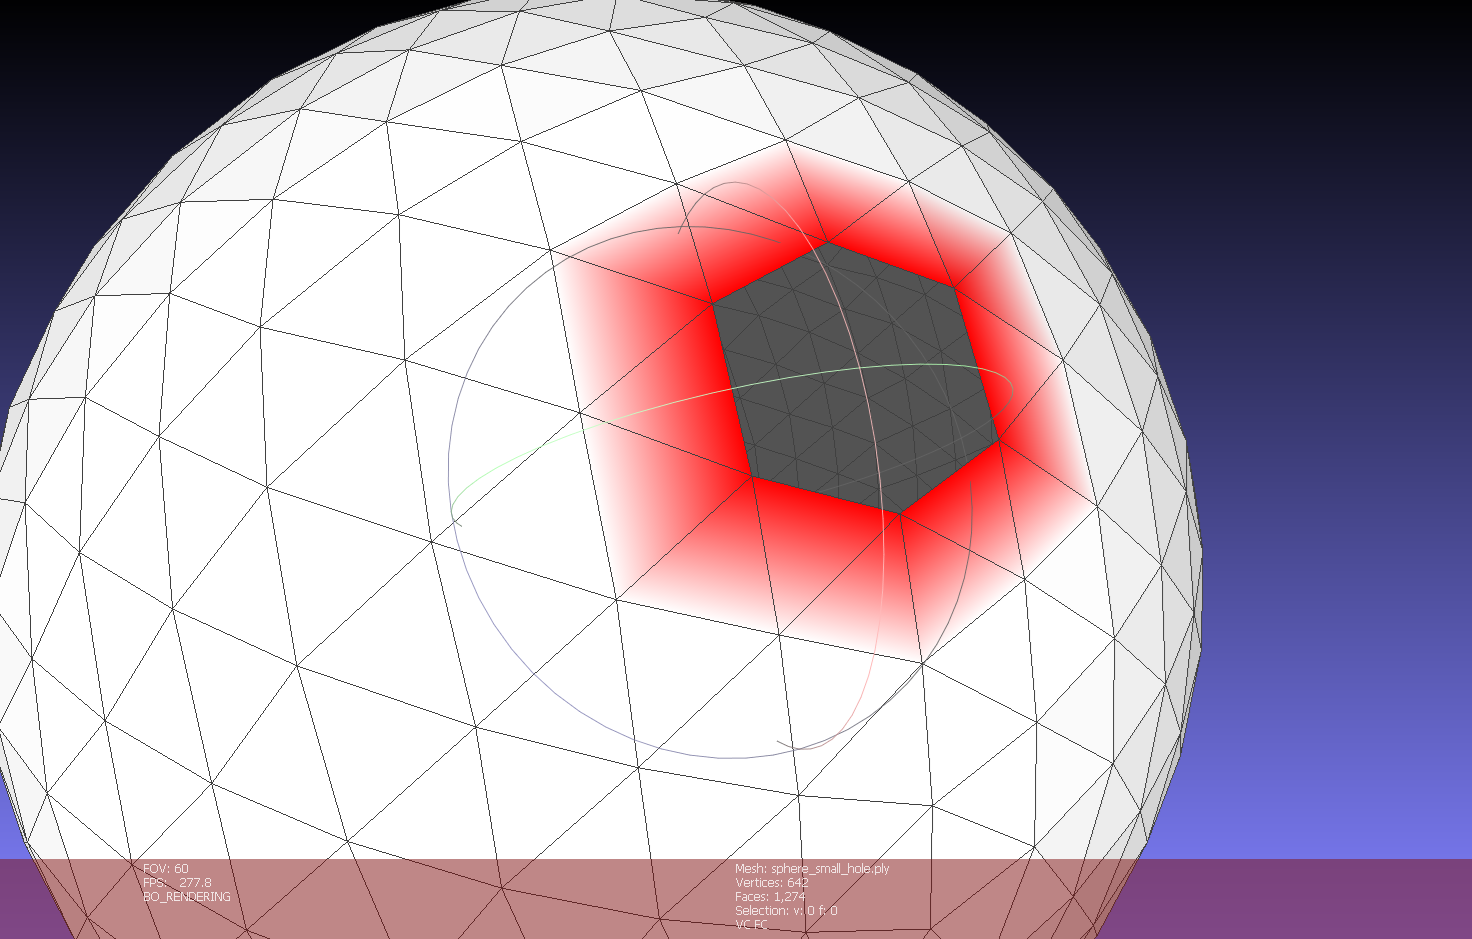
\includegraphics[width=0.45\textwidth]{figures/fig_dataset_sphere_small1.png}
    \hfill
    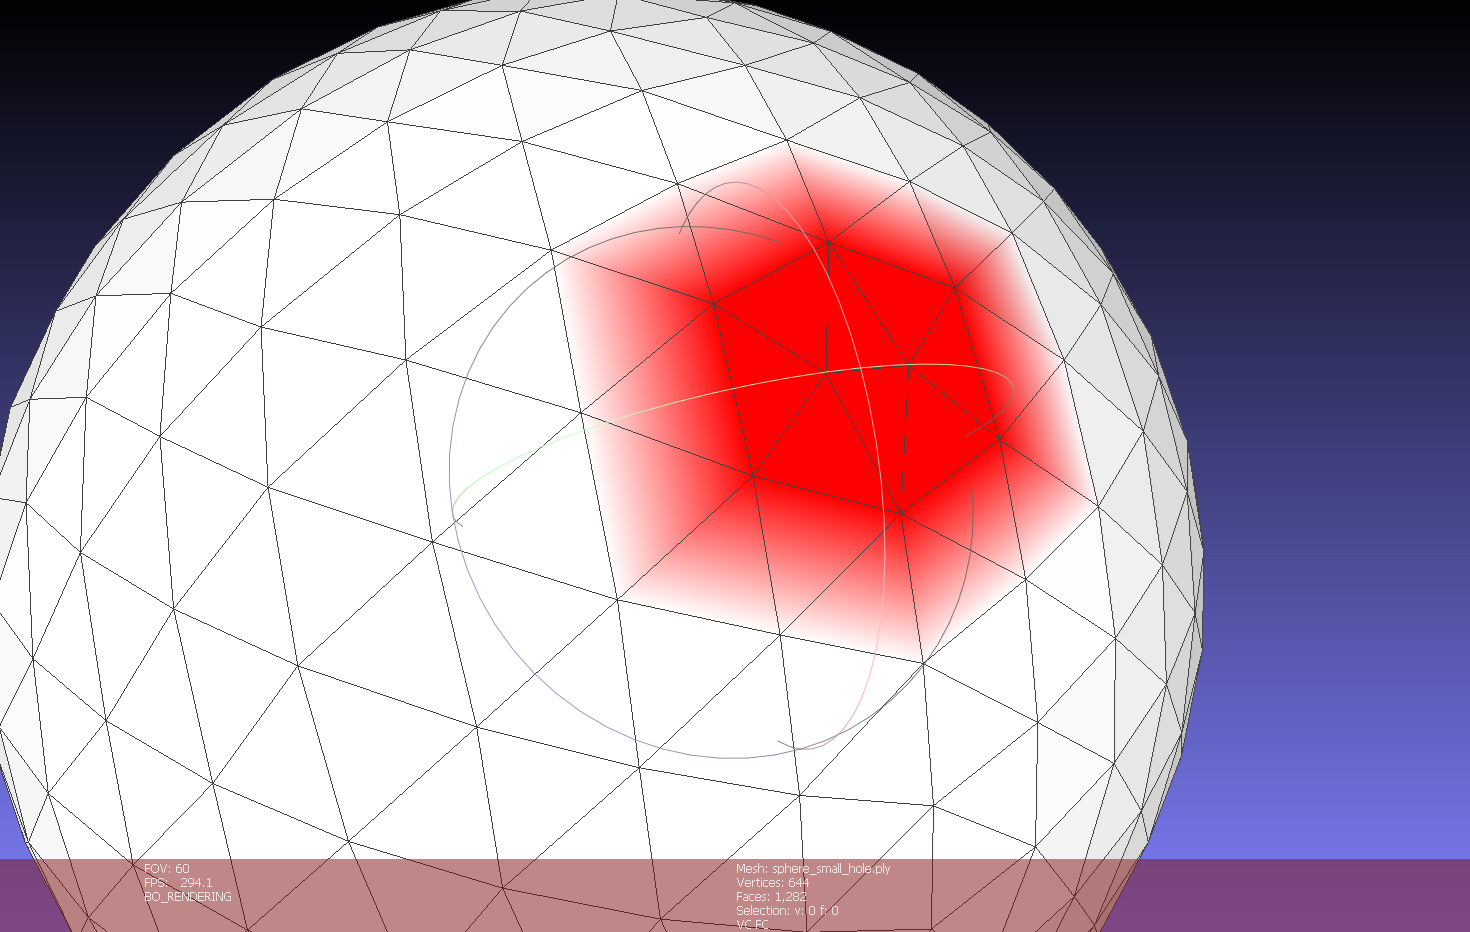
\includegraphics[width=0.45\textwidth]{figures/fig_dataset_sphere_small2.png}
    \caption{\texttt{sphere\_small}: input (left) and NFD result (right).}
    \label{fig:dataset-sphere-small}
\end{figure}

\begin{figure}[H]
    \centering
    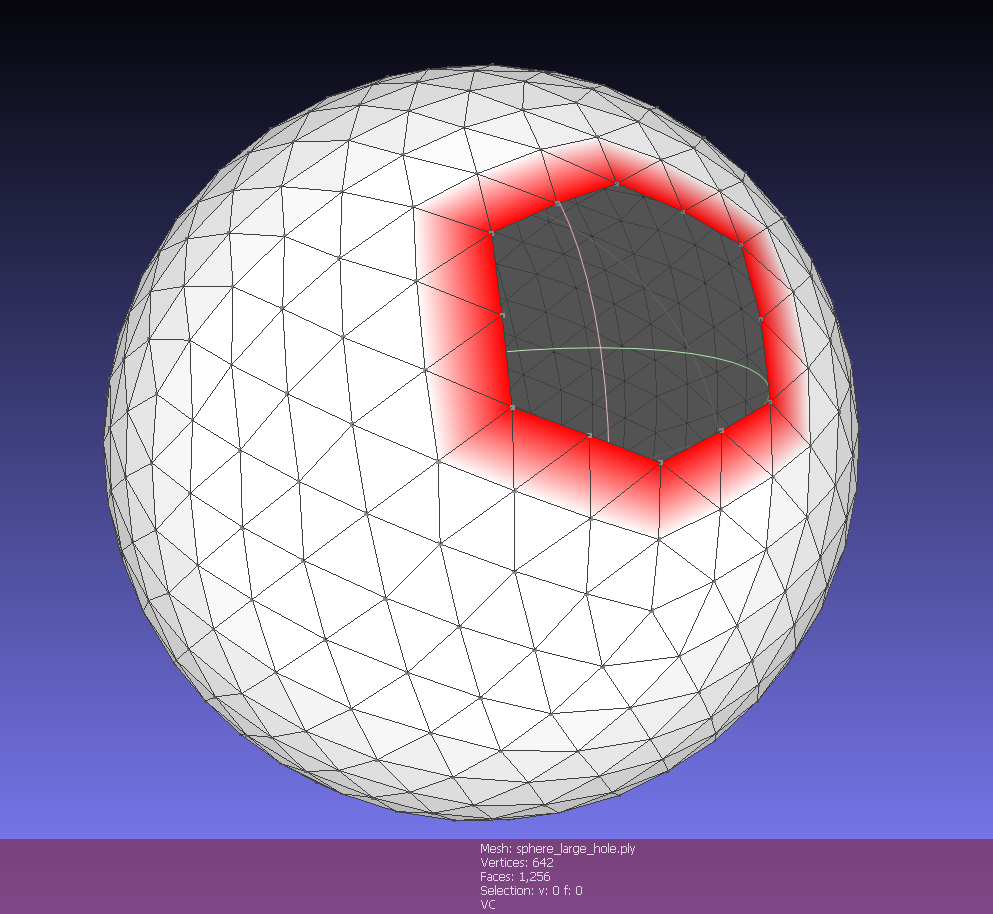
\includegraphics[width=0.45\textwidth]{figures/fig_dataset_sphere_large1.png}
    \hfill
    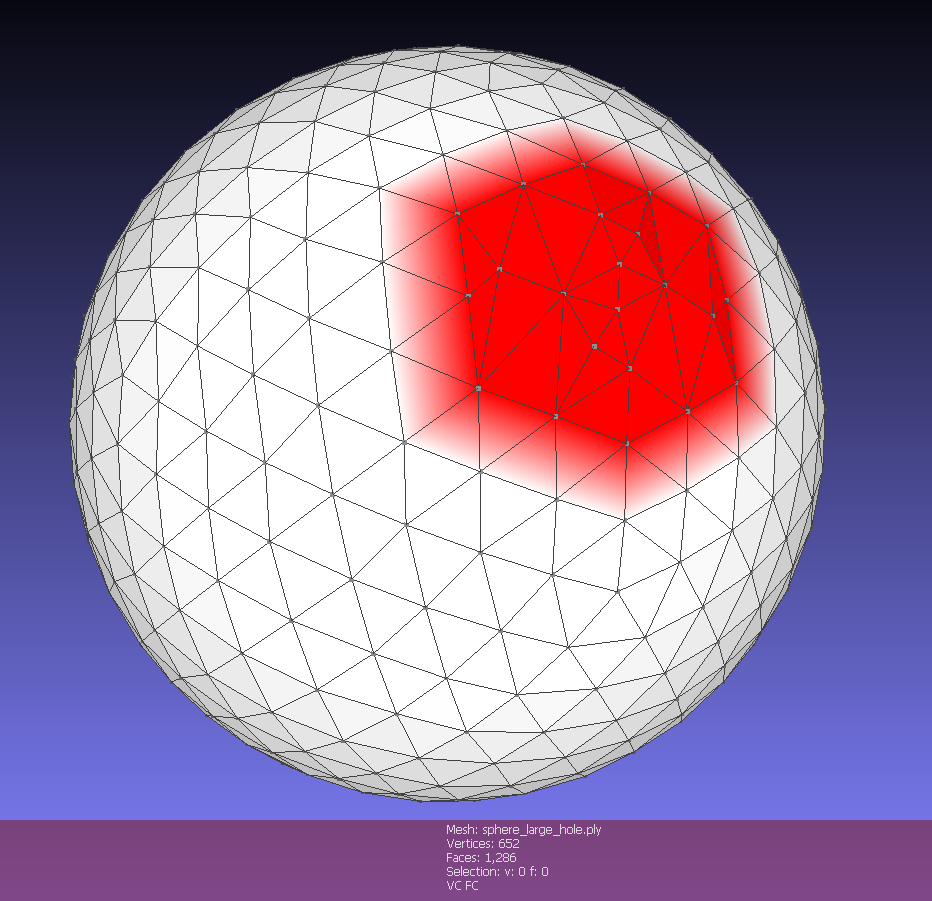
\includegraphics[width=0.45\textwidth]{figures/fig_dataset_sphere_large2.png}
    \caption{\texttt{sphere\_large}: input (left) and NFD result (right).}
    \label{fig:dataset-sphere-large}
\end{figure}

\begin{figure}[H]
    \centering
    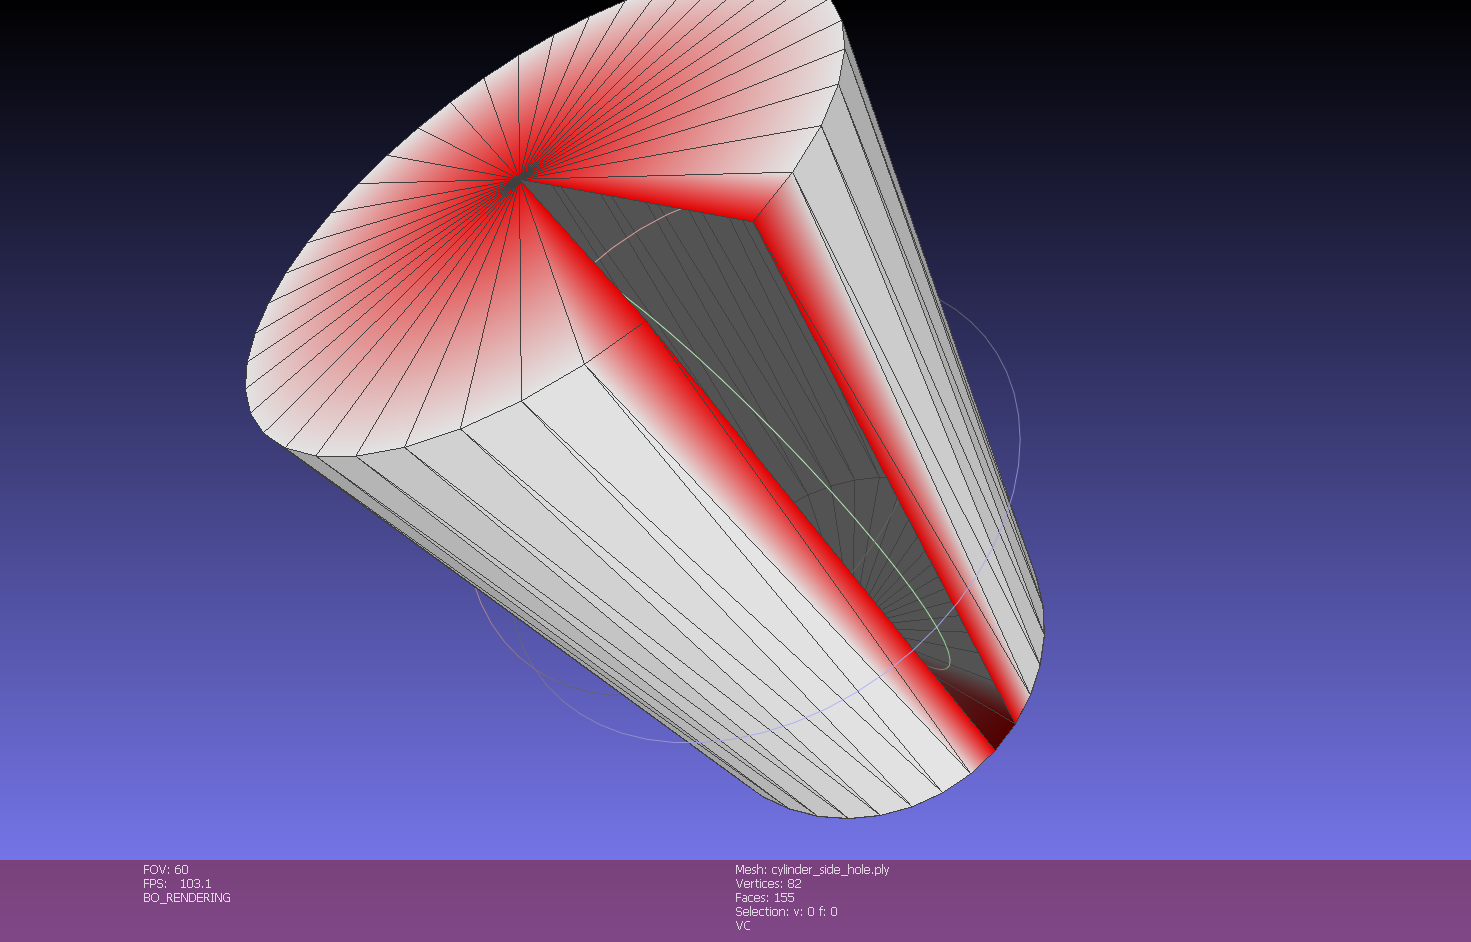
\includegraphics[width=0.45\textwidth]{figures/fig_dataset_cylinder1.png}
    \hfill
    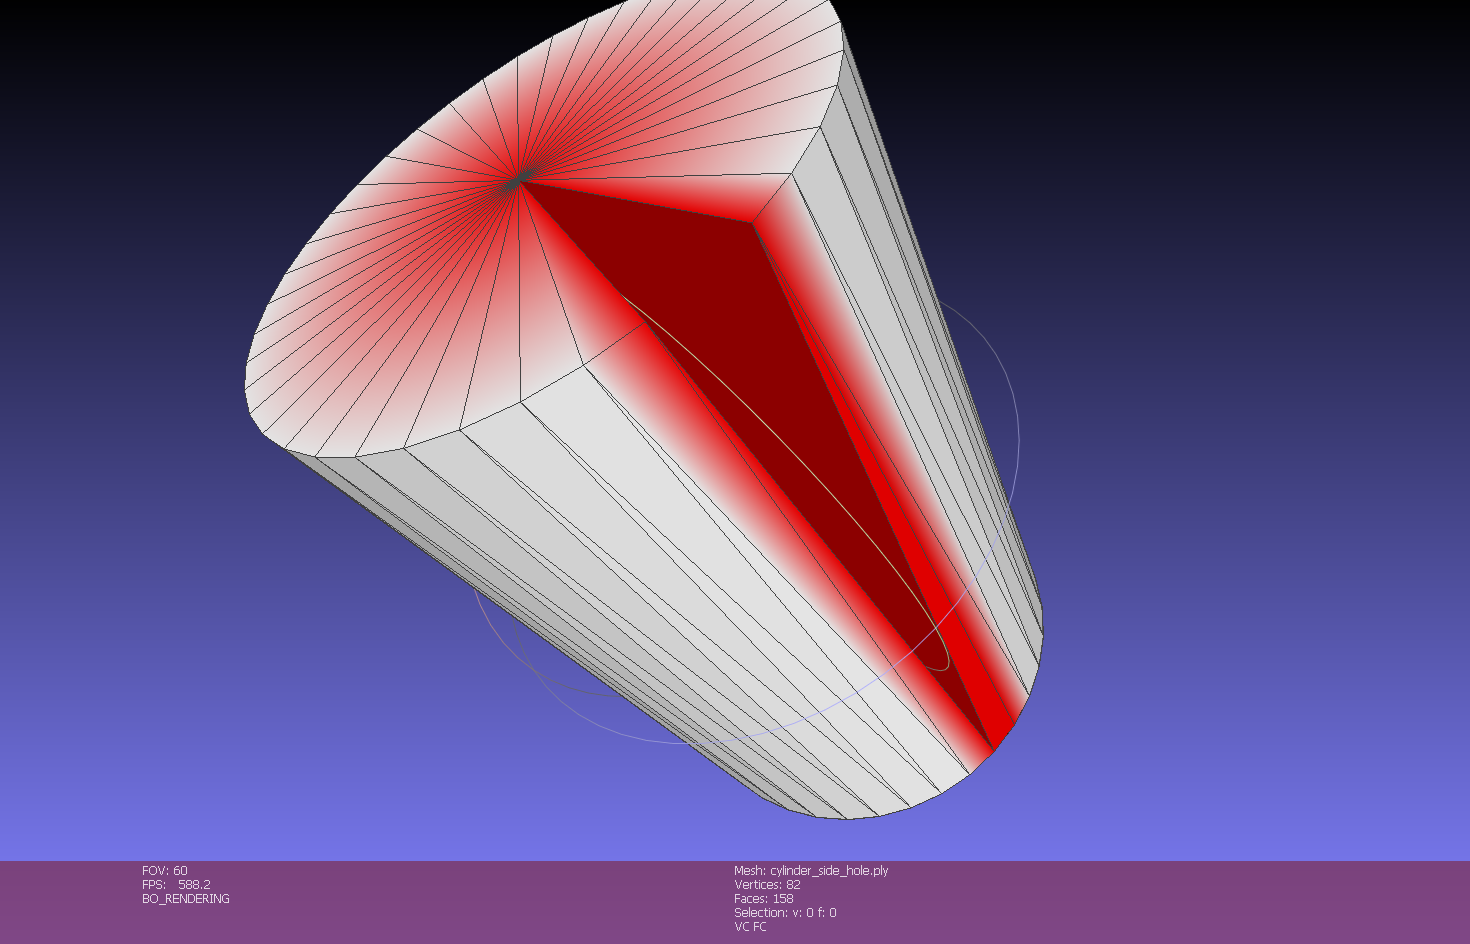
\includegraphics[width=0.45\textwidth]{figures/fig_dataset_cylinder2.png}
    \caption{\texttt{cylinder\_side}: input (left) and NFD result (right).}
    \label{fig:dataset-cylinder}
\end{figure}

\begin{figure}[H]
    \centering
    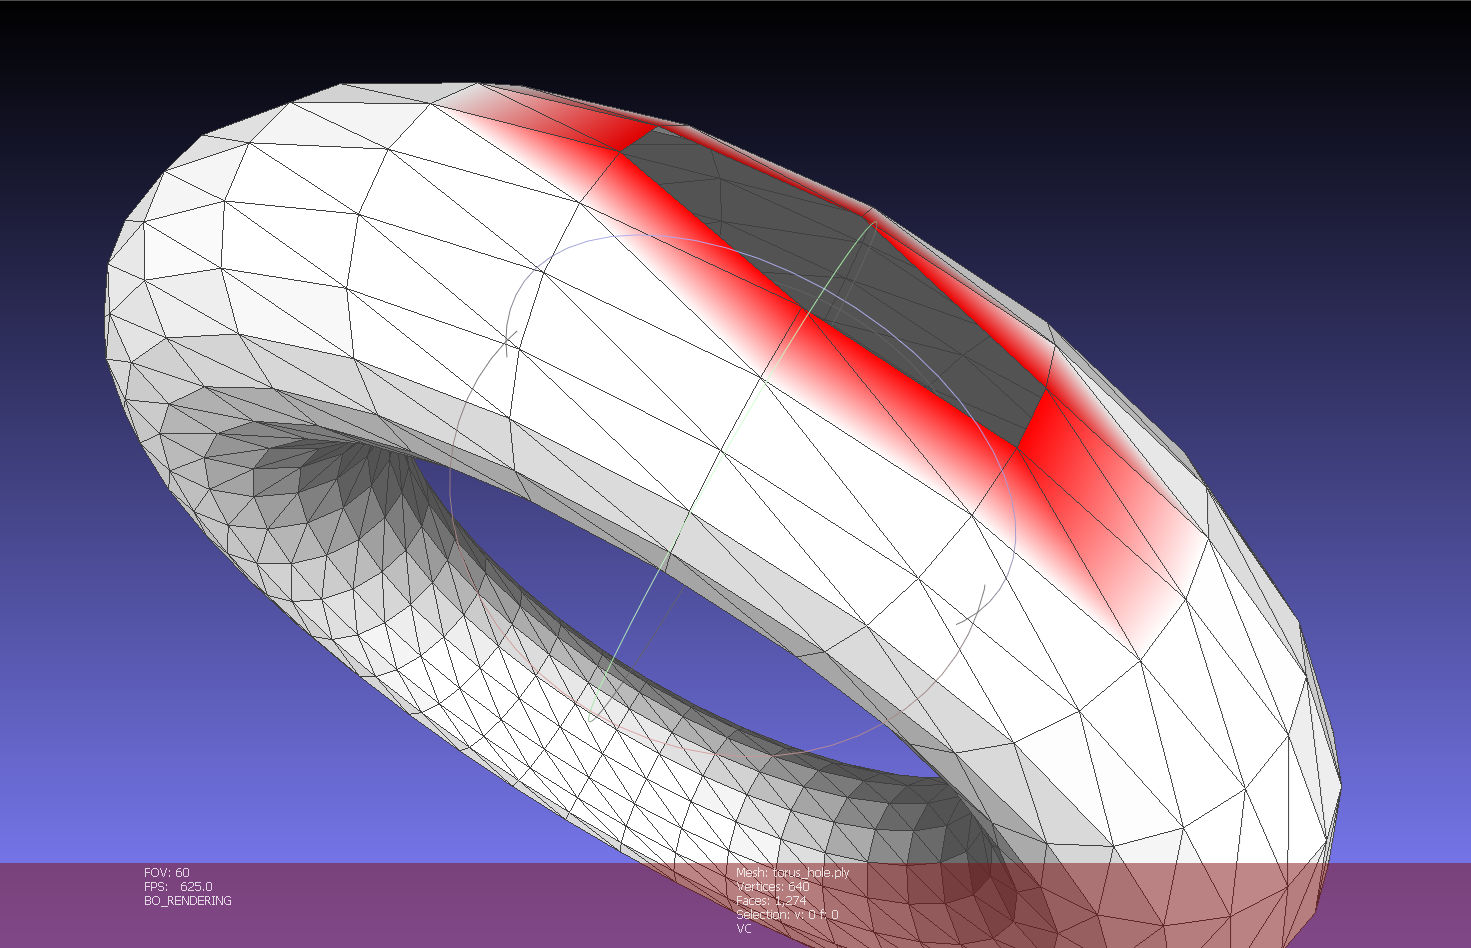
\includegraphics[width=0.45\textwidth]{figures/fig_dataset_torus1.png}
    \hfill
    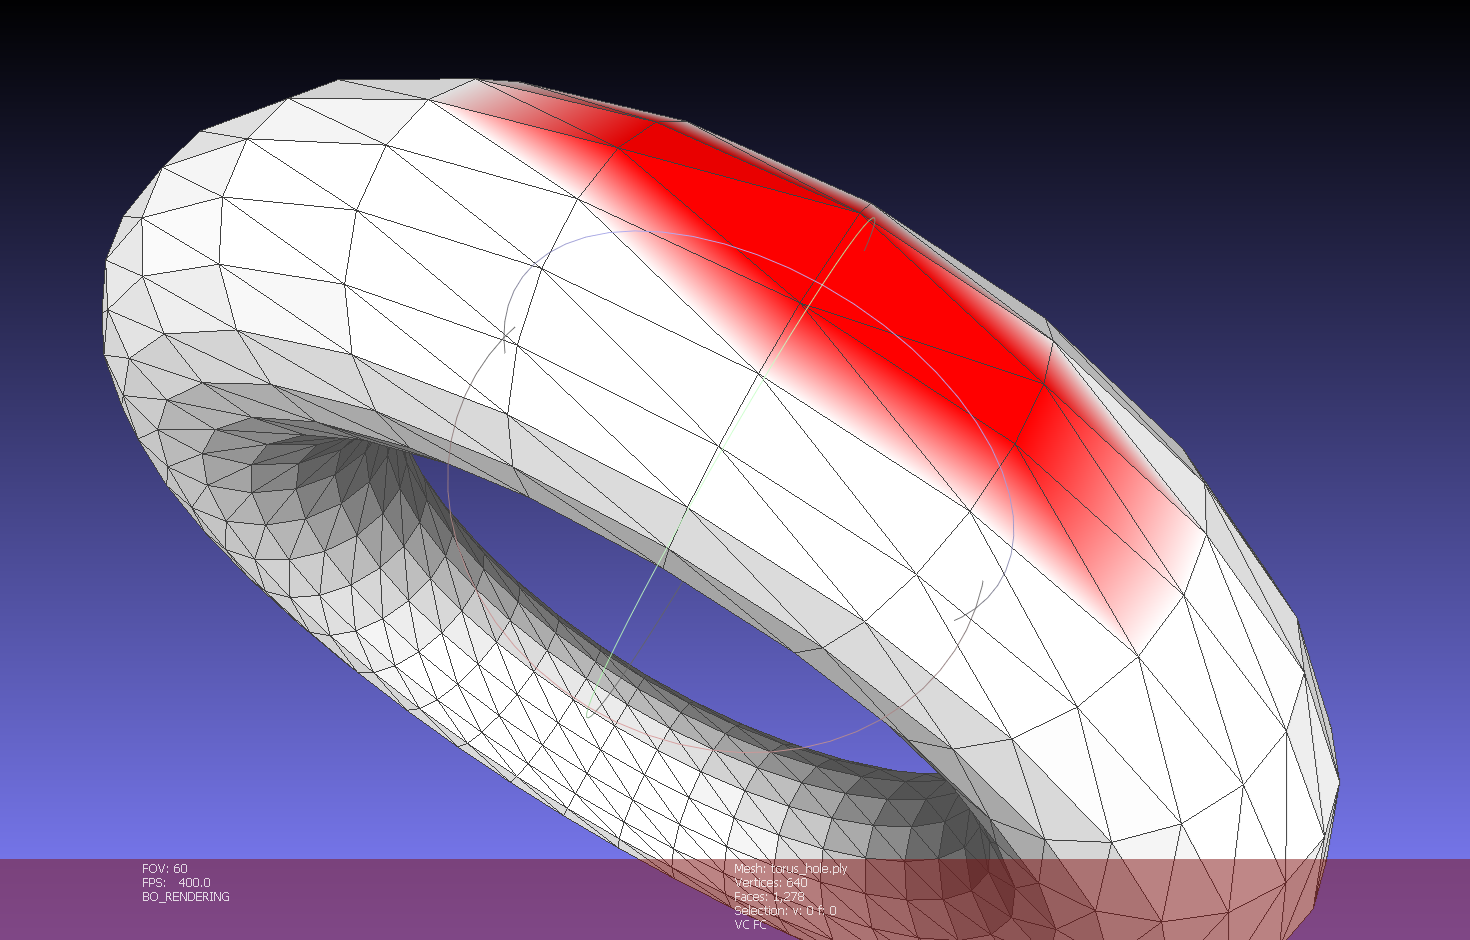
\includegraphics[width=0.45\textwidth]{figures/fig_dataset_torus2.png}
    \caption{\texttt{torus}: input (left) and NFD result (right).}
    \label{fig:dataset-torus}
\end{figure}

\begin{figure}[H]
    \centering
    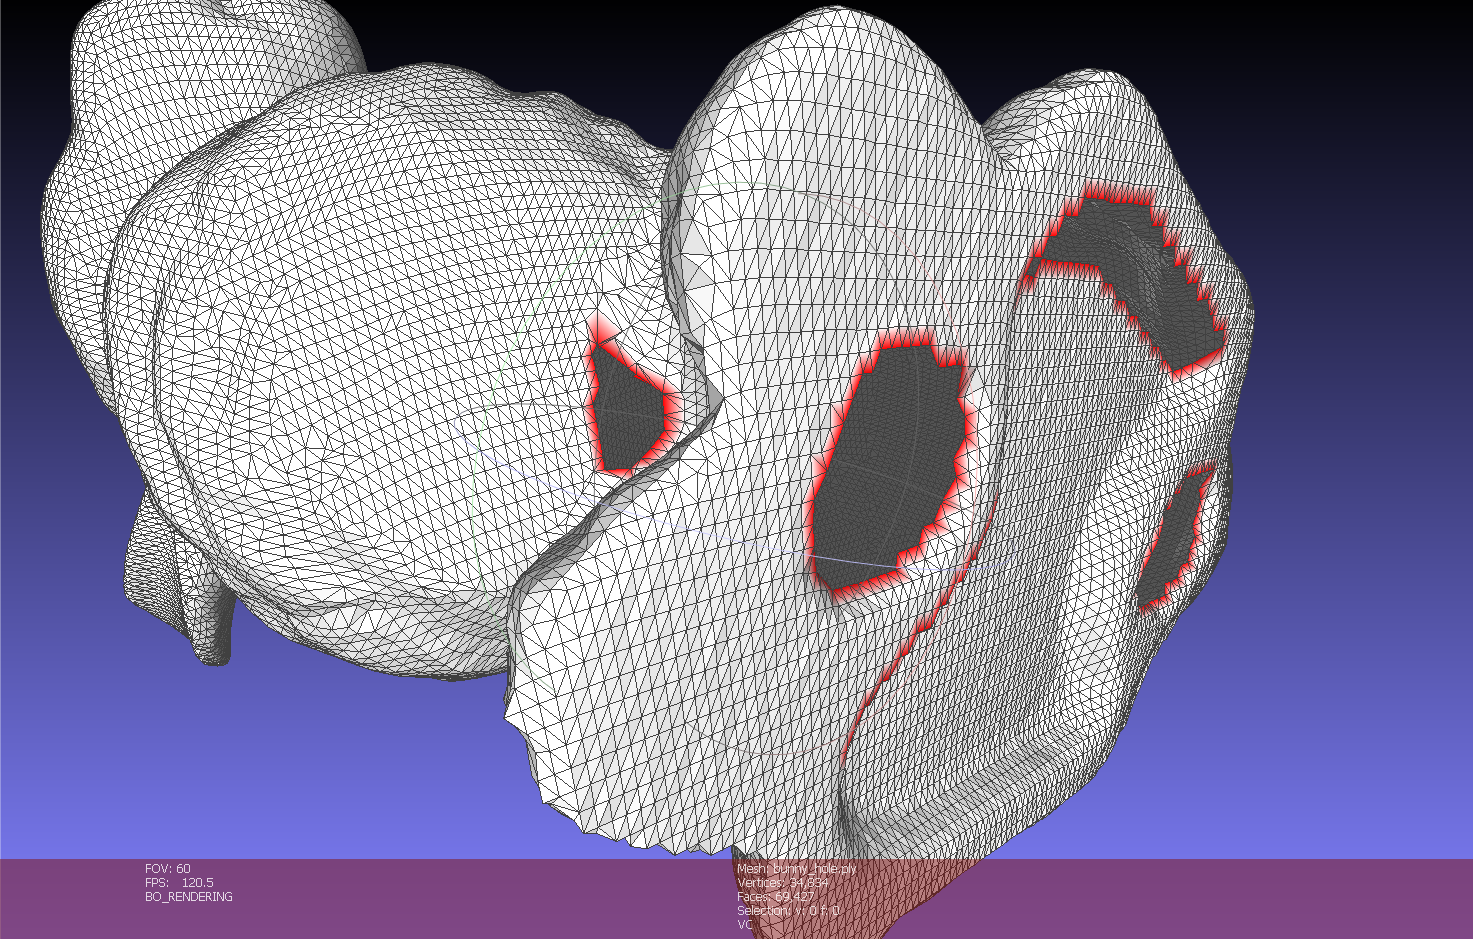
\includegraphics[width=0.45\textwidth]{figures/fig_dataset_bunny1.png}
    \hfill
    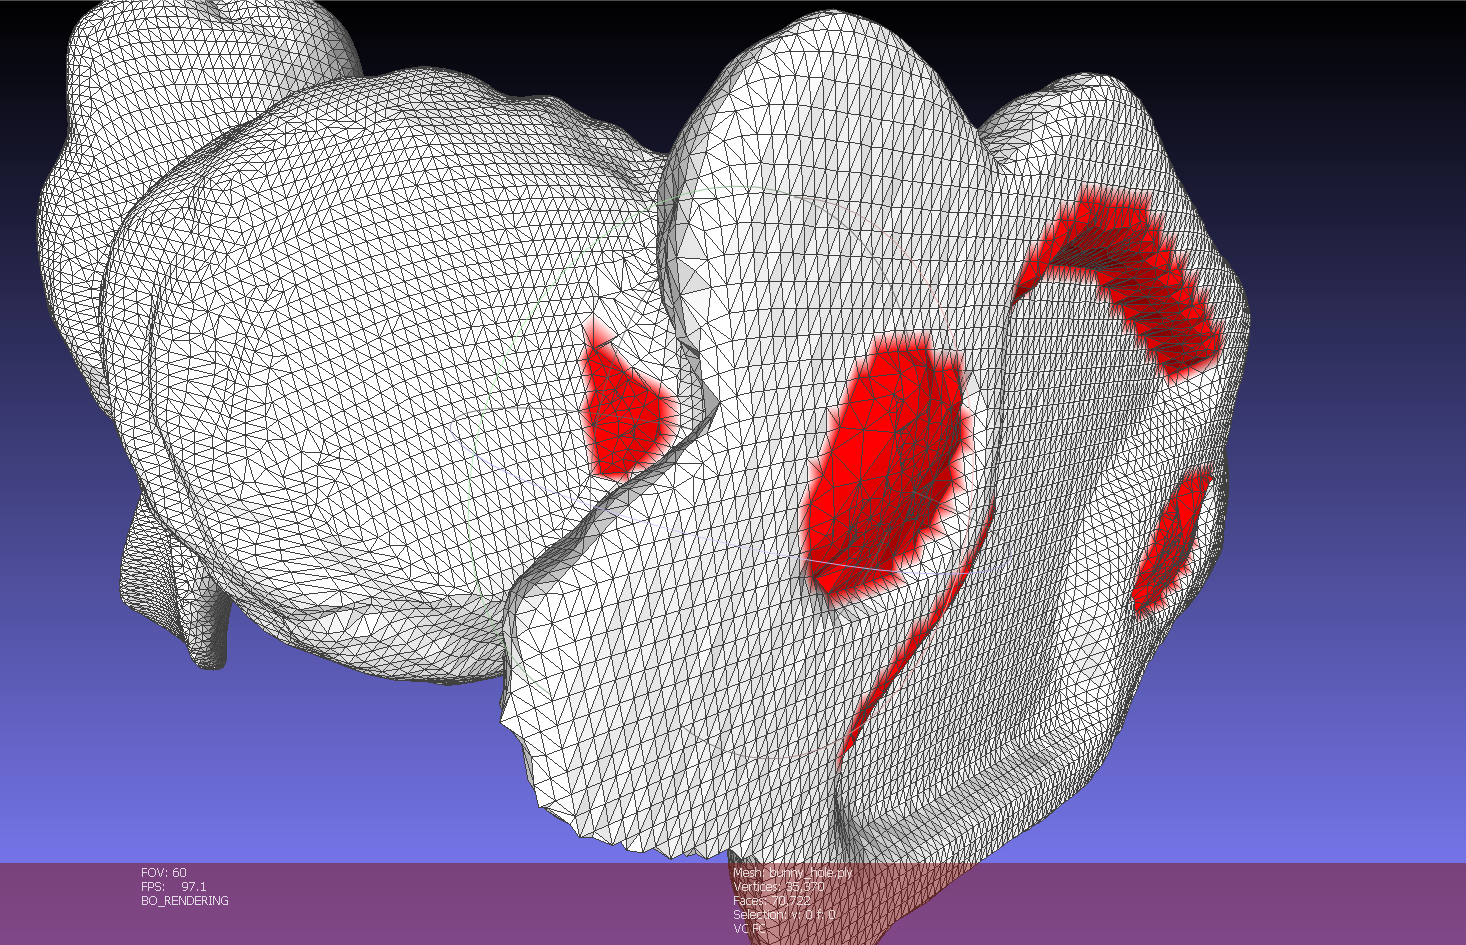
\includegraphics[width=0.45\textwidth]{figures/fig_dataset_bunny2.png}
    \caption{Stanford \texttt{bunny}: six holes (left) all filled (right).}
    \label{fig:dataset-bunny}
\end{figure}

\begin{figure}[H]
    \centering
    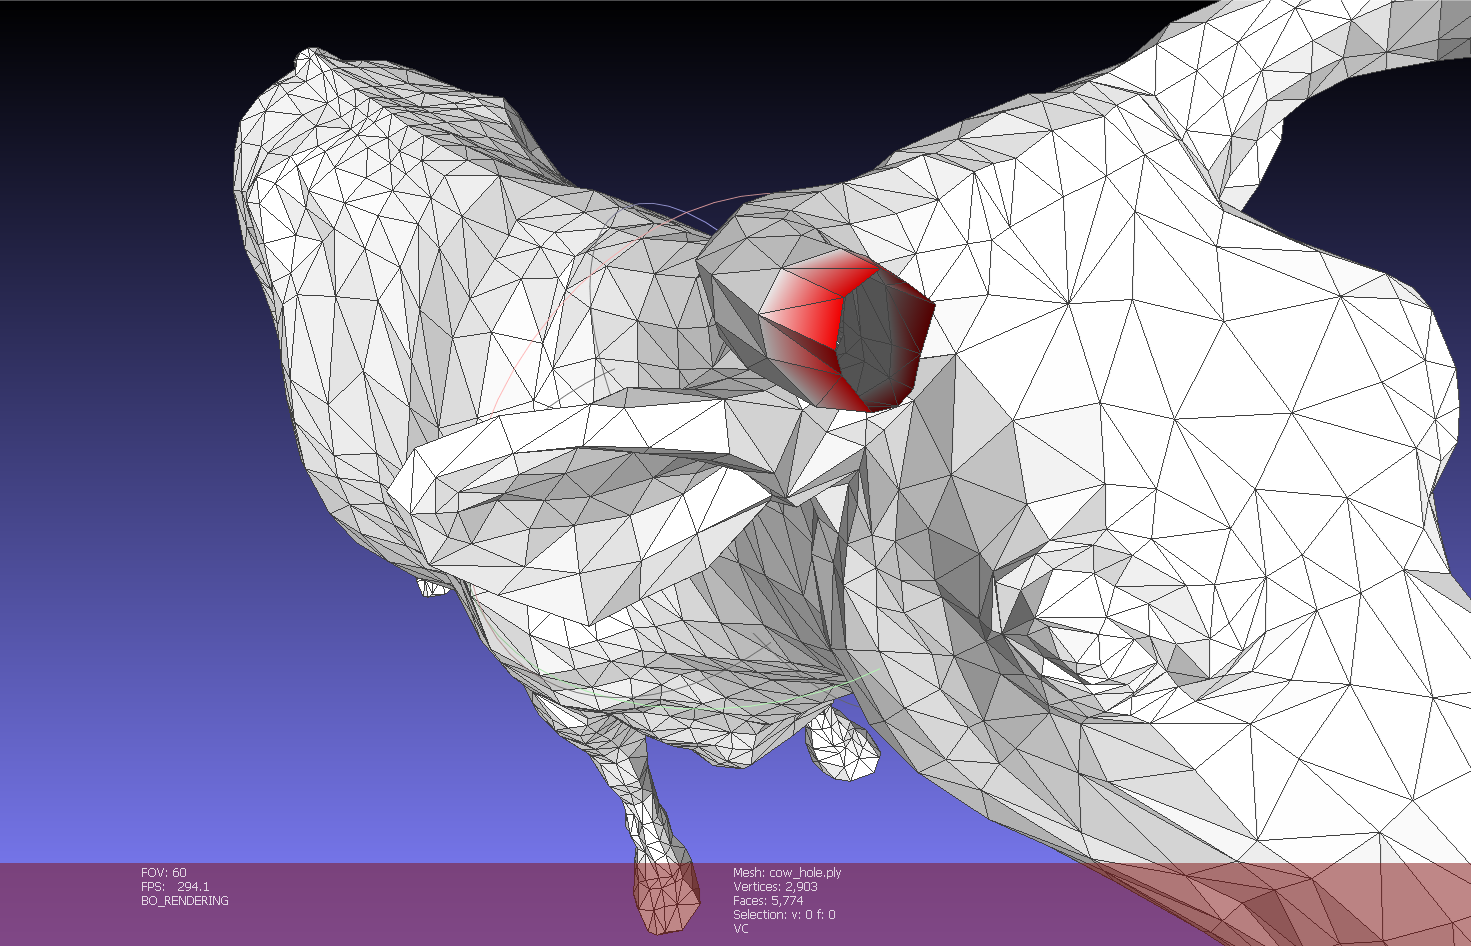
\includegraphics[width=0.45\textwidth]{figures/fig_dataset_cow1.png}
    \hfill
    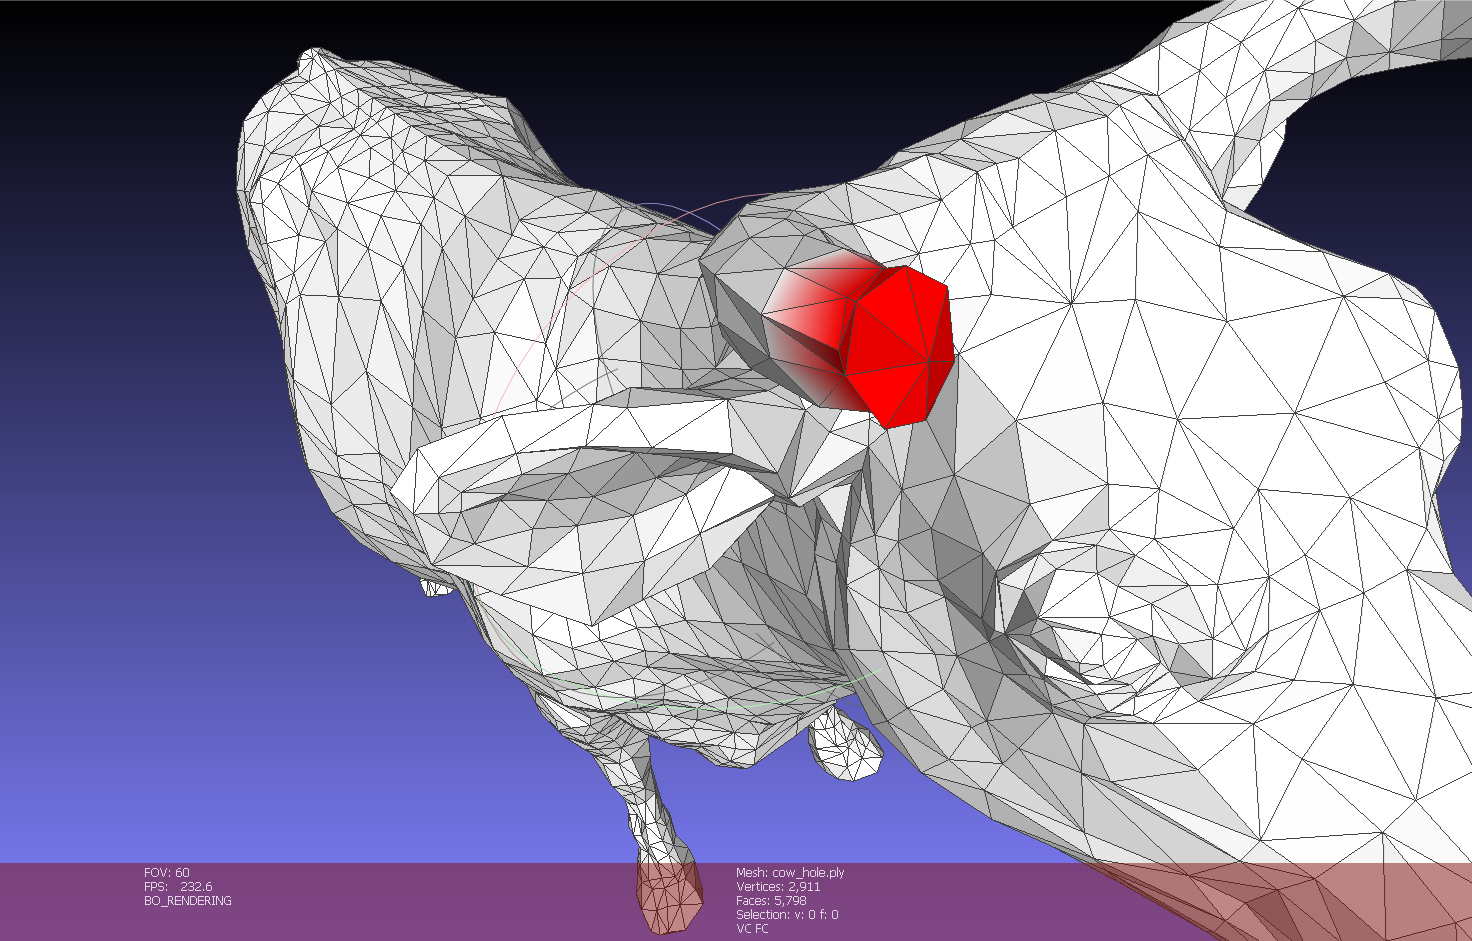
\includegraphics[width=0.45\textwidth]{figures/fig_dataset_cow2.png}
    \caption{\texttt{cow}: input (left) and NFD result (right).}
    \label{fig:dataset-cow}
\end{figure}

\section{Comparison with MeshLab Close Holes}

\begin{figure}[H]
    \centering
    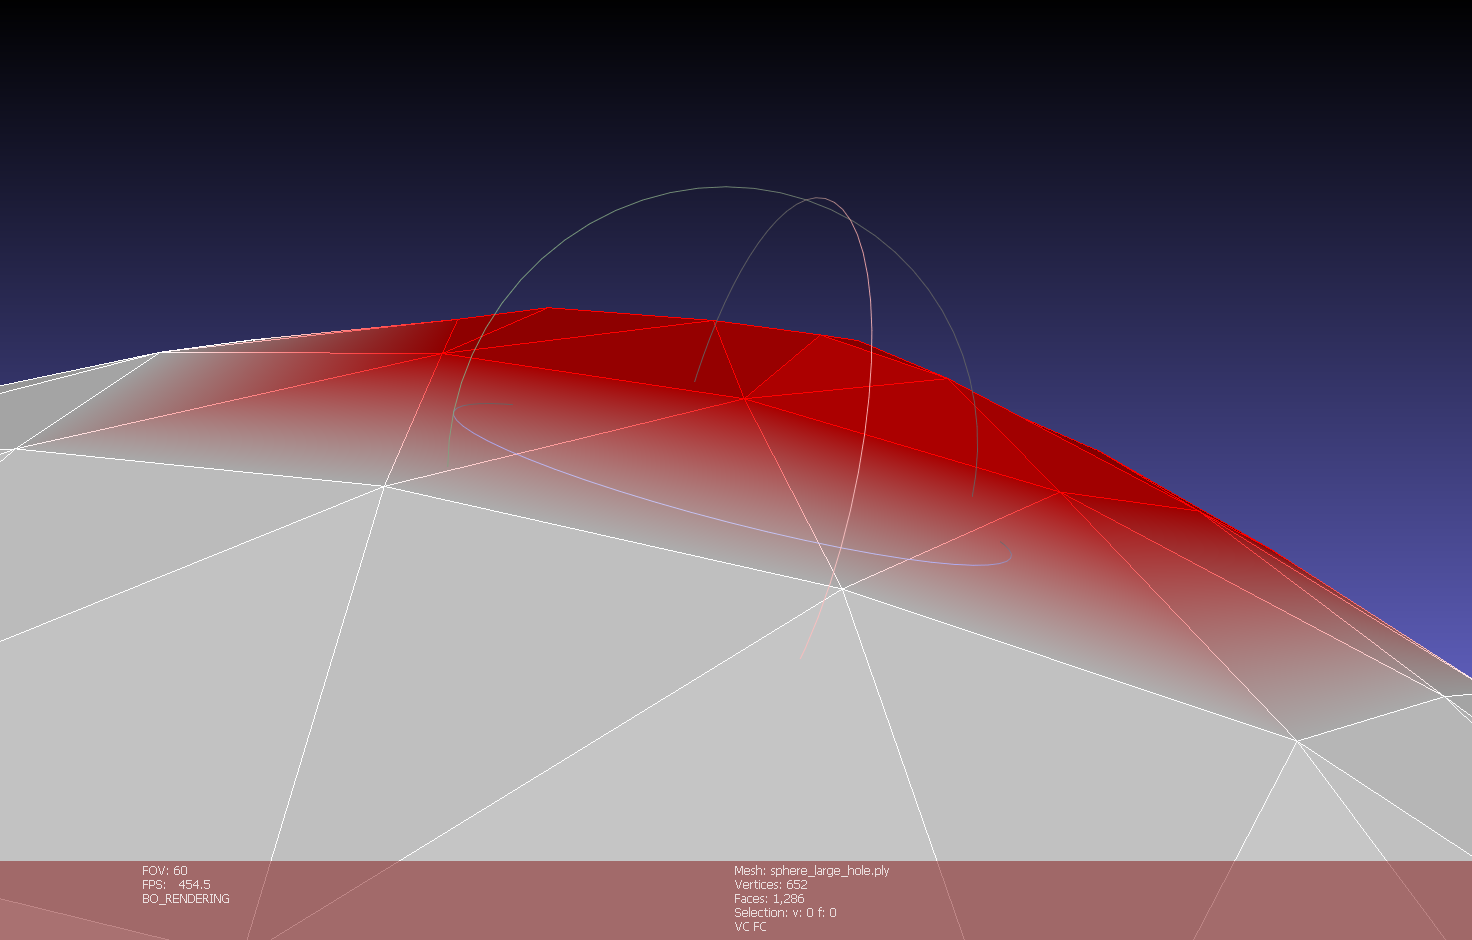
\includegraphics[width=0.45\textwidth]{figures/fig_compare_nfd_closeholes1.png}
    \hfill
    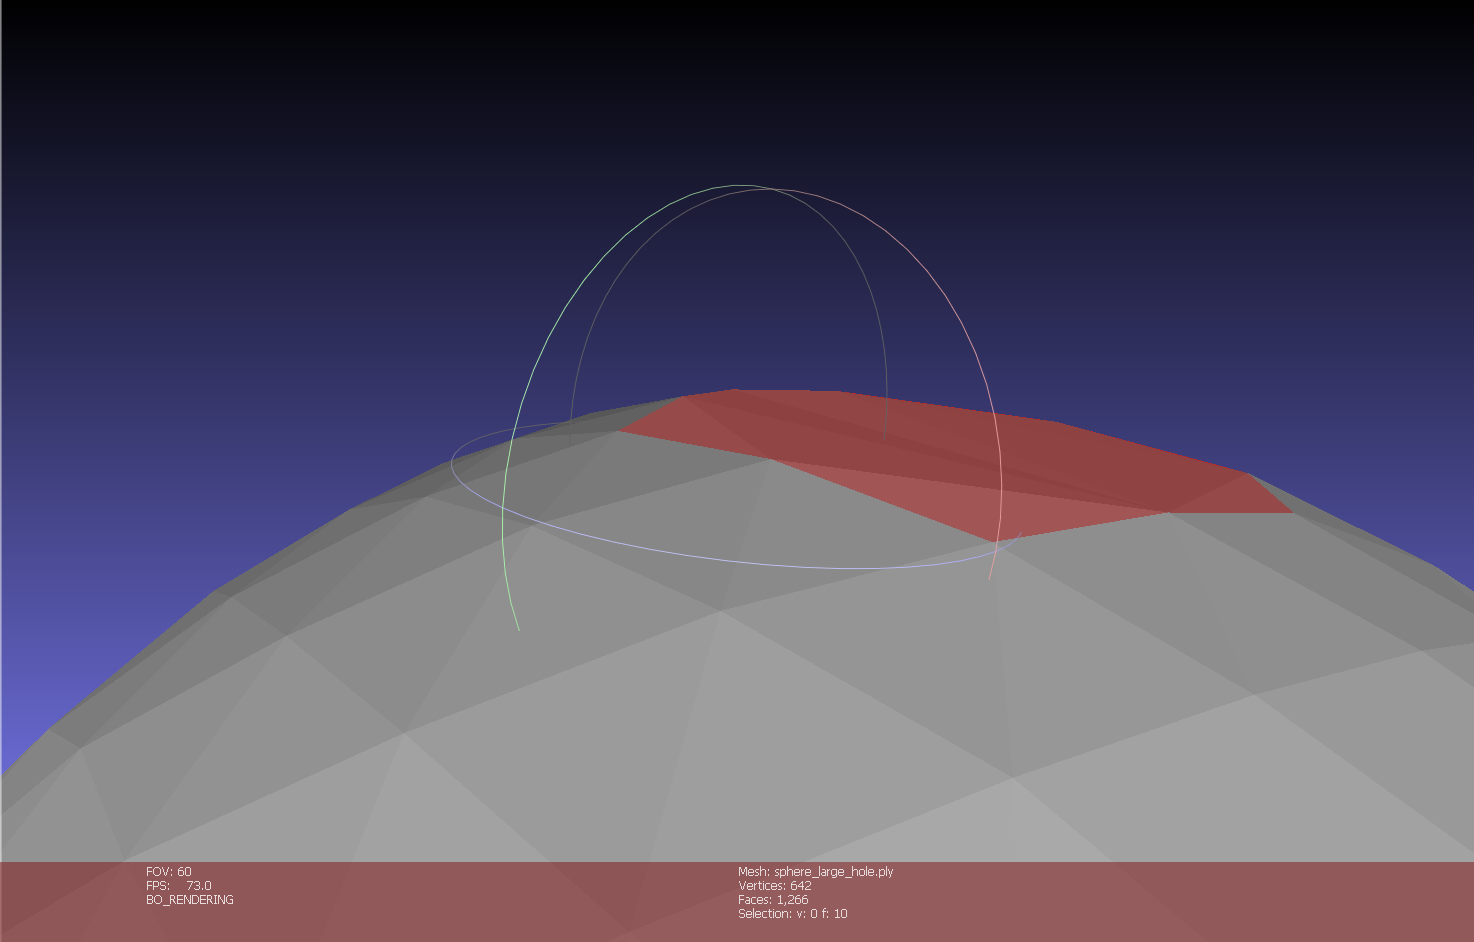
\includegraphics[width=0.45\textwidth]{figures/fig_compare_nfd_closeholes2.png}
    \caption{NFD (left) versus MeshLab \texttt{Close Holes} (right) on the same input.}
    \label{fig:compare-closeholes}
\end{figure}

The visual difference is most pronounced on convex inputs. \texttt{Close Holes} produces a planar triangulation that reads as a flat cap, while NFD bends the patch to follow the surrounding curvature. On a flat region (the side of a cylinder, for instance) the two outputs converge, which is consistent with the model: when $\theta \to 0$ in (\ref{eq:cap-height}), $h \to 0$ and the NFD displacement vanishes.

Figure~\ref{fig:delaunay-compare} shows the effect of the Delaunay-flip pass in Stage~3. Without flipping, slivers from ear clipping are clearly visible near the boundary; with flipping the tessellation becomes regular.

\begin{figure}[H]
    \centering
    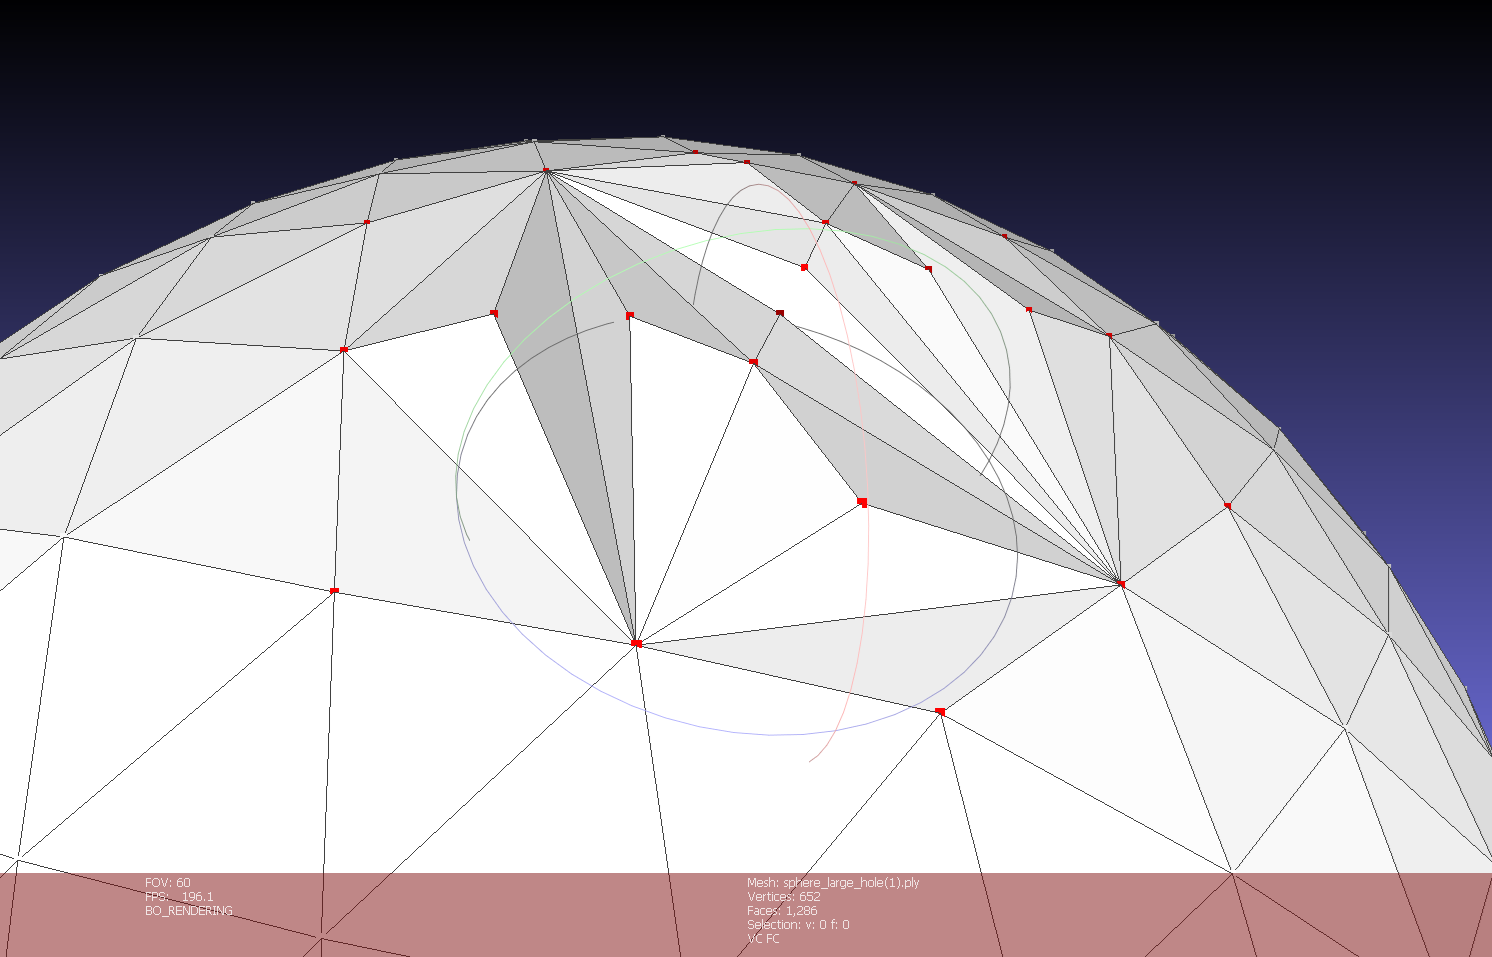
\includegraphics[width=0.45\textwidth]{figures/delaunay_off.png}
    \hfill
    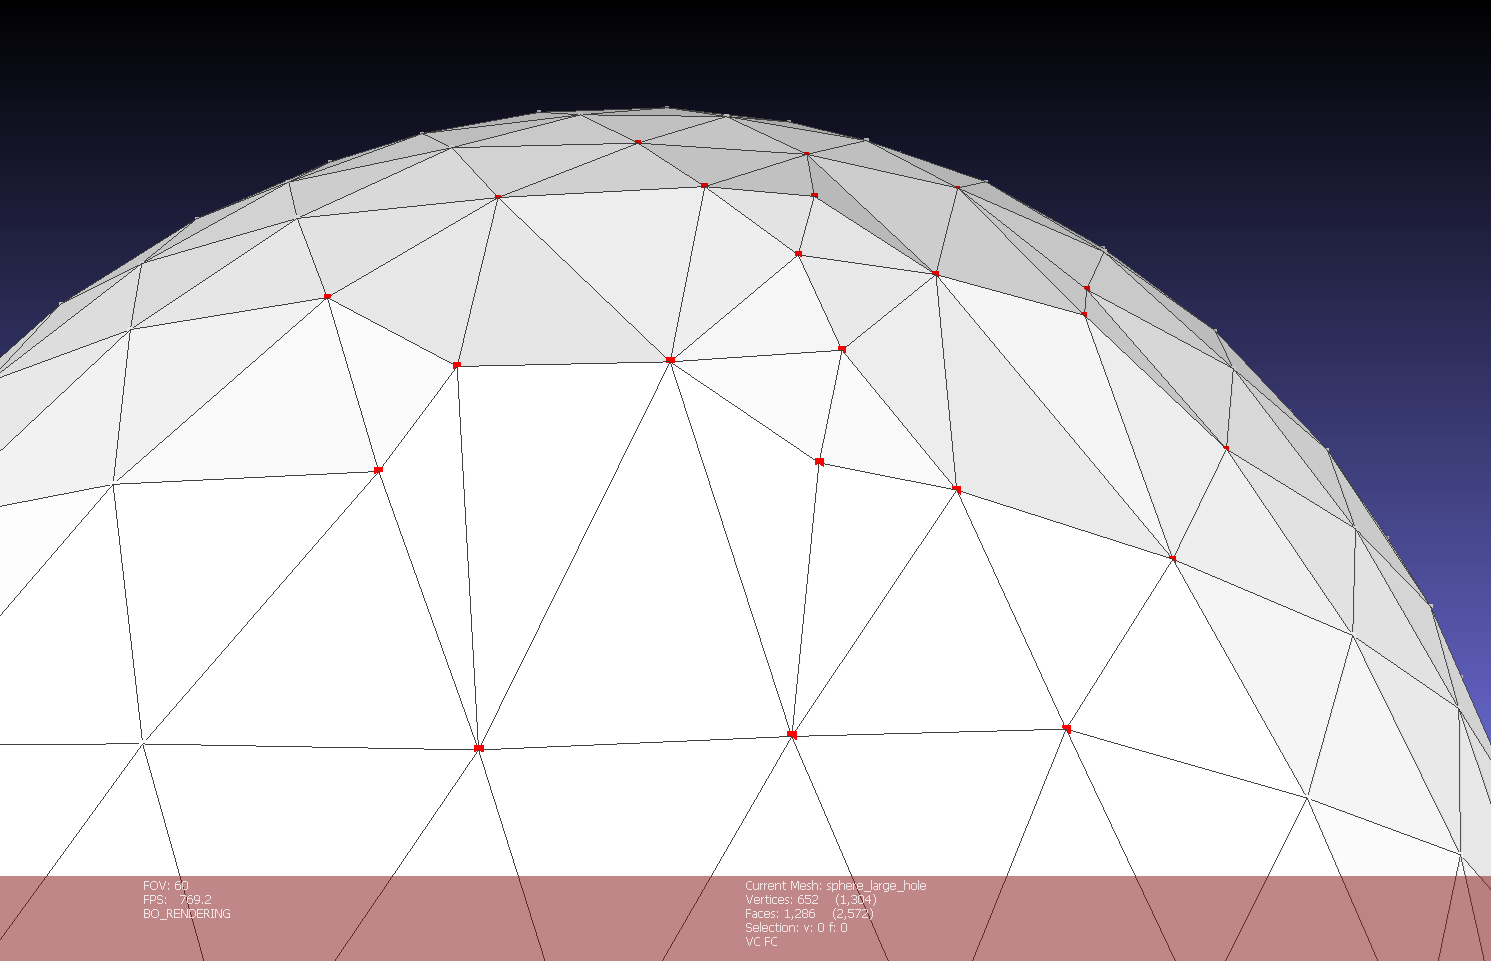
\includegraphics[width=0.45\textwidth]{figures/delaunay_on.png}
    \caption{Ear clipping without (left) and with (right) Delaunay edge flipping.}
    \label{fig:delaunay-compare}
\end{figure}

\section{Performance}

Wall-clock timings on a single thread of an Intel Core i7-12700H, averaged over five runs:

\begin{table}[H]
\centering
\caption{Single-threaded timings.}
\label{tab:timings}
\begin{tabularx}{\textwidth}{l r r X}
\toprule
\textbf{Model} & \textbf{Hole size} & \textbf{Total} & \textbf{Dominant stage} \\
\midrule
\texttt{sphere\_small} & 30 edges & 45 ms  & Stage 3 (triangulation) \\
\texttt{sphere\_large} & 80 edges & 210 ms & Stage 4 (factorisation + solves) \\
\texttt{bunny} (6 holes) & $\sim\!40$ each & 890 ms & sum over six patches \\
\bottomrule
\end{tabularx}
\end{table}

Stage~4 takes 40--60\% of the total on medium holes; the $LDL^T$ factorisation is the single most expensive step but is amortised over 50 solves. Stage~3 takes another 20--30\%, mostly because of the second Delaunay flip pass after centroid refinement. The remaining stages contribute negligibly. All runs complete in well under one second per hole, which is acceptable for interactive use inside MeshLab.
